\documentclass[11pt]{article}

%%%%%%%%%%%%%%%%%%%
% Page Layout
%%%%%%%%%%%%%%%%%%%

\setlength{\paperwidth}{8.5in} \setlength{\paperheight}{11in}
\setlength{\marginparwidth}{0in} \setlength{\marginparsep}{0in}
\setlength{\oddsidemargin}{0in} \setlength{\evensidemargin}{0in}
\setlength{\textwidth}{6.5in} \setlength{\topmargin}{-0.5in}
\setlength{\textheight}{9in}

%%%%%%%%%%%%%%%%%%%%%%%%%%%%%%%%%%%
% Include Packages and Style Files
%%%%%%%%%%%%%%%%%%%%%%%%%%%%%%%%%%%

\usepackage[english]{babel}
\usepackage{amsmath,amssymb,amsthm}
\usepackage{enumerate}
\usepackage{xcolor}
\usepackage[useregional]{datetime2}
\usepackage[pdftex]{graphicx,color}
\usepackage{graphicx}
\graphicspath{ {M5600/} }
\usepackage{multicol}
\setlength{\columnsep}{1.5cm}

%%%%%%%%%%%%%%%%%%%%%%%%%%%%%%
% Define theorem environments
%%%%%%%%%%%%%%%%%%%%%%%%%%%%%%

\newtheorem{theorem}{Theorem}[section]
\newtheorem{proposition}[theorem]{Proposition}
\newtheorem{lemma}[theorem]{Lemma}
\newtheorem{corollary}[theorem]{Corollary}
\newtheorem{claim}[theorem]{Claim}
\newtheorem{question}[theorem]{Question}
\newtheorem{conjecture}[theorem]{Conjecture}

\theoremstyle{definition}
\newtheorem{definition}[theorem]{Definition}
\newtheorem{example}[theorem]{Example}
\newtheorem*{remark}{Remark}

%%%%%%%%%%%%%%%%%%%%%%
% Define new commands
%%%%%%%%%%%%%%%%%%%%%%

\newcommand{\R}{\mathbb{R}}


\newcommand{\E}{\mathbb{E}}
\renewcommand{\P}{\mathbb{P}}
\newcommand{\Var}{\operatorname{Var}}
\newcommand{\1}[1]{\mathbf{1} \left \{ #1 \right \}}
\newcommand{\Range}{\operatorname{Range}}

%%%%%%%%%%%%%%%%%%%%%%

\begin{document}

\title{Numerical Analysis Project \\ MATH 5600 \\ Homework 1}
\date{Due: February 10, 2021}
\author{Authors: \\ Dane Gollero \\ Ike Griss Salas \\ Magon Bowling}

\maketitle

\section*{\textbf{Models of the Earth with Respect to Coordinate Systems}}
In our work through the term project, we utilize two coordinate systems: Geographical and Cartesian.  Geographical coordinates are used to identify a location on the Earth in terms of Longitude and Latitude.  In relationship with Cartesian coordinates, Geographic coordinates rotate around the z-axis with respect to time.  At time = 0, the x-axis intersects the globe at the Equator and Prime Meridian.  The y-axis therefore perpendicular to the xz-plane.
\[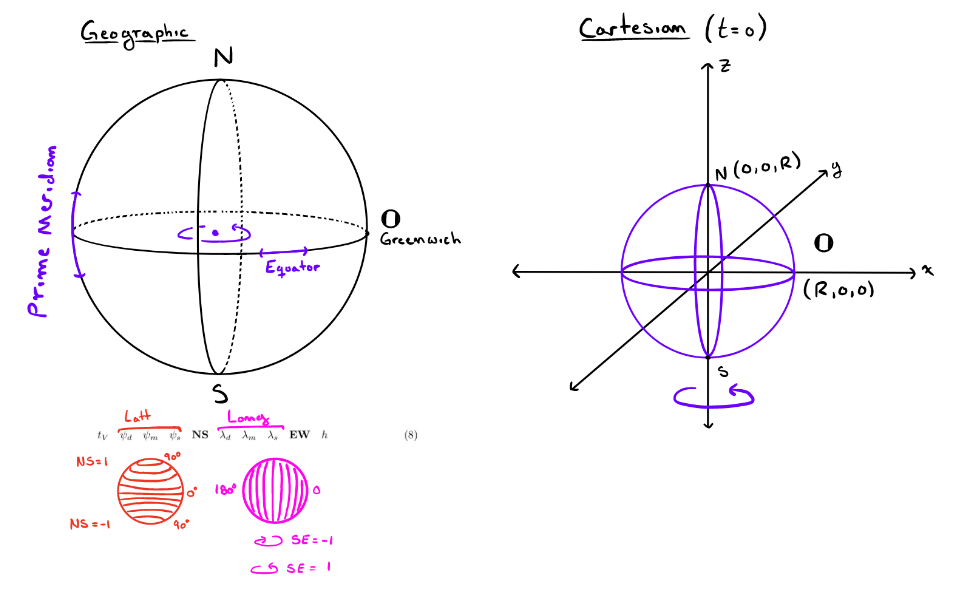
\includegraphics[width=15cm, height=9cm]{M5600/Images/M5600_EarthModels.PNG}\]

\begin{itemize}
\item[{\textbf{Exercise 1:}}] Find a formula that describes the trajectory of the point \textbf{O} in Cartesian coordinates as a function of time.
\end{itemize}
From Physics, we know that distance is equal to the rate of an object multiplied by the time traveled.  We can apply this to trajectory with the equation $\theta = \omega \cdot t$, where $\omega$ is angular velocity.  Angular velocity is the distance around the globe divided by one sidereal day.  Thus we obtain the angle $\theta = \frac{2\pi}{s} \cdot t$.  The formula that describes the trajectory of the point \textbf{O} as a function of time in Cartesian coordinates is: \\
\[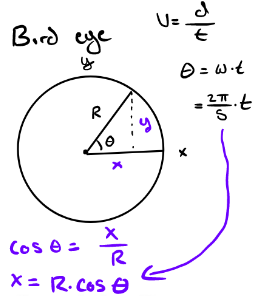
\includegraphics[width=0.15\textwidth]{M5600/Images/M5600_theta_2pi_s.PNG}\]
\[\textbf{O}_{car}(t) =
\begin{bmatrix}
R \cos{\big(\frac{2pi}{s}\big) \cdot t} \\
R \sin{\big(\frac{2pi}{s}\big) \cdot t} \\
0 \end{bmatrix} \]

\begin{itemize}
\item[{\textbf{Exercise 2:}}] Write a program that converts angles from degrees, minutes, and seconds to radians, and vice versa.
\end{itemize}
\[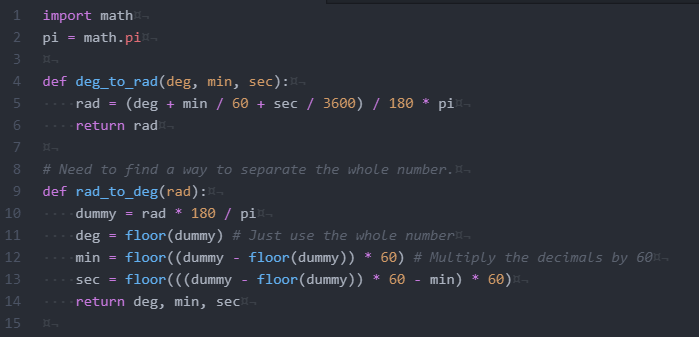
\includegraphics{Images/M5600_2_Code.PNG}\]

\begin{itemize}
\item[{\textbf{Exercise 3:}}] Find a formula that converts position as given in (8) at time $t = 0$ into Cartesian coordinates.
\end{itemize}
It is important to note the parameters for the following variables: \\
\(t_V = 0, \quad \psi_d, \psi_m, \psi_s \in \big[0, \frac{pi}{2}\big], \quad \textrm{NS} \in \{-1, 1\}, \quad \lambda_d, \lambda_m, \lambda_s \in [o, \pi], \quad \textrm{EW} \in \{-1, 1\}, \quad h = h\)

\begin{itemize}
\item[{\textbf{Step 1)}}] Using the program from \textbf{Exercise 2}, we will do the following conversions: \\
\(\psi_d, \psi_m, \psi_s \ \textrm{to} \ \phi \in \big[0, \frac{pi}{2}\big]\) \qquad and \qquad \(\lambda_d, \lambda_m, \lambda_s \ \textrm{to} \ \theta \in [o, \pi]\)

\item[{\textbf{Step 2)}}] We will solve for $x, \ y, \ \textrm{and} \ z$ using trigonometry functions.  Note the following diagrams, where \textbf{R} is the radius of the Earth, $\alpha$ is the perpendicular distance of the position, and the rest have been identified above:
\end{itemize}
\[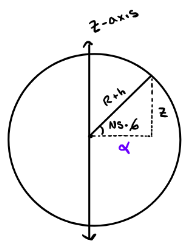
\includegraphics[width=0.22\textheight]{Images/M5600_3.1.PNG} \hspace{2cm} 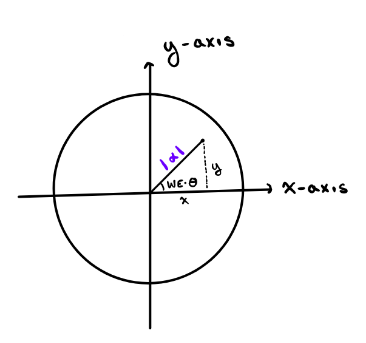
\includegraphics{Images/M5600_3.2.PNG}\]
We arrive at the following three equations:
\begin{itemize}
\begin{multicols}{2}
    \item \(z(\phi, \textrm{NS}, h) = (R + h) \sin (\textrm{NS} \cdot \phi)\)
    \item \(\alpha(\phi, \textrm{NS}, h) = (R + h) \cos (\textrm{NS} \cdot \phi)\)
    \item \(x(\theta, \textrm{EW}, \alpha) = |\alpha| \cos (\textrm{EW} \cdot \theta)\)
    \item \(y(\theta, \textrm{EW}, \alpha) = |\alpha| \sin (\textrm{EW} \cdot \theta) \)
\end{multicols}
\end{itemize}
Thus Given we know $\phi$ and $\theta$ using the program from \textbf{Exercise 2}, we have at $t=0$,
\[(8):= \textbf{X}_o = \begin{bmatrix} x \\ y \\ z \end{bmatrix} = \begin{bmatrix}
|\alpha| \cos (\textrm{EW} \cdot \theta) \\ |\alpha| \sin (\textrm{EW} \cdot \theta) \\ (R + h) \sin (\textrm{NS} \cdot \phi) \end{bmatrix}\]

\begin{itemize}
\item[{\textbf{Exercise 4:}}] Find a formula that converts position and general time $t$ as a given in (8) into Cartesian coordinates.
\end{itemize}
We use our formula from \textbf{Exercise 3} to find the Cartesian coordinates at $t=0$ and then use a rotation matrix to find position at time $t$.  It is important to note that the rotation is around the $z$-axis.

\[\textrm{Rotation Matrix:} \quad R(t) = \begin{bmatrix}
\cos \big(\frac{2\pi}{s} \cdot t\big) & -\sin \big(\frac{2\pi}{s} \cdot t\big) & 0 \\ \sin \big(\frac{2\pi}{s} \cdot t\big) & \cos \big(\frac{2\pi}{s} \cdot t\big) & 0 \\ 0 & 0 & 1 \end{bmatrix}\] \\
We compure the following matrix multiplication,
\[\textbf{X(t)} = \begin{bmatrix} x(t) \\ y(t) \\ z(t) \end{bmatrix} = R(t) \cdot \textbf{x}_o\]
\\
\[\textbf{X(t)} = \begin{bmatrix}
\cos \big(\frac{2\pi}{s} \cdot t\big) & -\sin \big(\frac{2\pi}{s} \cdot t\big) & 0 \\ \sin \big(\frac{2\pi}{s} \cdot t\big) & \cos \big(\frac{2\pi}{s} \cdot t\big) & 0 \\ 0 & 0 & 1 \end{bmatrix} \cdot
\begin{bmatrix}
|\alpha| \cos (\textrm{EW} \cdot \theta) \\
|\alpha| \sin (\textrm{EW} \cdot \theta) \\
(R + h) \sin (\textrm{NS} \cdot \phi)
\end{bmatrix} \] \\
Now we arrive at,

\[\textbf{X(t)} = \begin{bmatrix}
|\alpha| \cos \big(\frac{2\pi}{s} \cdot t \big) \cos (\textrm{EW} \cdot \theta) - |\alpha| \sin \big(\frac{2\pi}{s} \cdot t \big) \sin (\textrm{EW} \cdot \theta) \\
|\alpha| \sin \big(\frac{2\pi}{s} \cdot t \big) \cos (\textrm{EW} \cdot \theta) + |\alpha| \cos \big(\frac{2\pi}{s} \cdot t \big) \sin (\textrm{EW} \cdot \theta) \\
(R + h) \sin (\textrm{NS} \cdot \phi)
\end{bmatrix} \]

\begin{itemize}
\item[{\textbf{Exercise 5:}}] Find a formula that converts a position given in Cartesian coordinates at time $t=0$ into a position of the form (8).
\end{itemize}
Given Cartesian coordinates \([x, y, z]^T\), we need to find Geographical coordinates in terms of \\
\(t_V \quad \psi_d \quad \psi_m \quad \psi_s \quad \textrm{NS} \quad \lambda_d \quad \lambda_m \quad \lambda_s \quad \textrm{EW} \quad h.\) \ Using the following diagrams, we can identify Geographic variables to assist in forming the formula for conversion.
\\
\[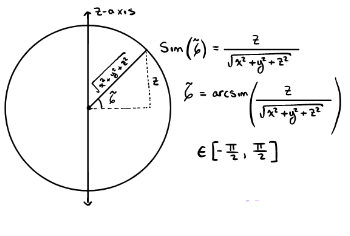
\includegraphics[width=0.35\textheight]{Images/M5600_5.1.PNG} 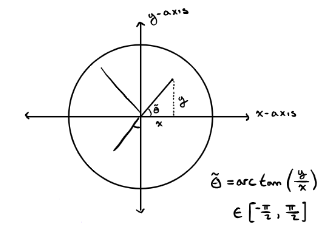
\includegraphics[width=0.35\textheight]{Images/M5600_5.2.PNG}\]
\begin{itemize}
    \item \(t_V = 0\)
    \item \(h = \sqrt{x^2 + y^2 + z^2} - R\)
    \item NS = \begin{cases}
    1,& \text{$z \geq 0$} \\ -1,& \text{$z>0$} \end{cases}
    \item \(\psi_d, \psi_m, \psi_s = \Bigg| \arcsin \Big(\frac{z}{\sqrt{x^2 + y^2 + z^2}}\Big) \Bigg| \quad \textrm{*Use conversion program} \rightarrow [\psi_d, \psi_m, \psi_s]\)
    \item EW = \begin{cases}
    1,& \text{$y \geq 0$} \\ -1,& \text{$y>0$} \end{cases}
    \item \(\lambda_d, \lambda_m, \lambda_s\) := \begin{cases}
    \frac{\pi}{2},& \text{$x = 0$} \\
    0,& \text{$x>0 \ \textrm{and} \ y=0$} \\
    \pi,& \text{$x<0 \ \textrm{and} \ y=0$} \\
    \arctan \big(\frac{y}{x}\big),& \text{$x>0 \ \textrm{and} \ y>0$} \\
    \big|\arctan \big(\frac{y}{x}\big)\big|,& \text{$x>0 \ \textrm{and} \ y<0$} \\
    \pi + \arctan \big(\frac{y}{x}\big),& \text{$x<0 \ \textrm{and} \ y>0$} \\
    \pi - \arctan \big(\frac{y}{x}\big),& \text{$x<0 \ \textrm{and} \ y<0$} \\
    \end{cases} \quad \textrm{*Use conversion program} \rightarrow \([\lambda_d, \lambda_m, \lambda_s]\)
\end{itemize}

\begin{itemize}
\item[{\textbf{Exercise 6:}}] Find a formula that converts general time $t$ and a position given in Cartesian coordinates into a position of the form (8).
\end{itemize}
\\
\begin{itemize}
\item[{\textbf{Exercise 7:}}] Find a formula that describes the trajectory of lamp post B12 in Cartesian coordinates as a function of time.
\end{itemize}
\begin{minipage}{0.6\linewidth}
Illustrated in the diagram at the right, we have a fixed point where street light B12 is located at the following Geographic coordinates:
\[t \quad 40 \quad 45 \quad 55.0 \quad 1 \quad 111 \quad 50 \quad 58.0 \quad -1 \quad 1372.00\]
We use the conversion program from \textbf{Exercise 2} to define $\psi$ and $\theta$, and then use the formula from \textbf{Exercise 4} to generate the formula we need.
\end{minipage} \qquad
\begin{minipage}{0.4\linewidth}
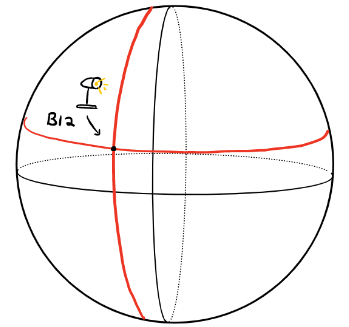
\includegraphics[width=0.2\textheight]{Images/M5600_7_light.PNG}
\end{minipage}
Define:
\begin{align*}
    \phi &= \phi(40, 45, 55.0) \\
    &= \bigg(40 + \frac{45}{60} + \frac{55.0}{3600}\bigg) \cdot \frac{\pi}{180}
\end{align*}
\begin{align*}
    \theta &= \theta(111, 50, 58.0) \\
    &= \bigg(111 + \frac{50}{60} + \frac{58.0}{3600}\bigg) \cdot \frac{\pi}{180}
\end{align*}
\\
\textbf{Exercise 4} formula:
\[\textbf{X}_{Lamp}(t+t_V) = \begin{bmatrix}
|\alpha| \cos \big(\frac{2\pi}{s} \cdot (t+t_V) \big) \cos (\textrm{EW} \cdot \theta) - |\alpha| \sin \big(\frac{2\pi}{s} \cdot (t+t_V) \big) \sin (\textrm{EW} \cdot \theta) \\
|\alpha| \sin \big(\frac{2\pi}{s} \cdot (t+t_V) \big) \cos (\textrm{EW} \cdot \theta) + |\alpha| \cos \big(\frac{2\pi}{s} \cdot (t+t_V) \big) \sin (\textrm{EW} \cdot \theta) \\
(R + h) \sin (\textrm{NS} \cdot \phi)
\end{bmatrix}\] \\
where \(\alpha = (R + h) \cos (\textrm{NS} \cdot \phi)\).



\end{document}
